\section{The Quantum Fourier Transform and its Applications}

\textbf{5.1}

We have \[U = \frac{1}{\sqrt{N}}\sum_{j=0}^{N-1}\sum_{k=0}^{N-1}e^{2\pi i jk/N}\ket{k}\bra{j}\] and
\[U^\dag = \frac{1}{\sqrt{N}}\sum_{j=0}^{N-1}\sum_{k=0}^{N-1}e^{-2\pi i jk/N}\ket{j}\bra{k}\]
This means 
\[U^\dag U = \left(\frac{1}{\sqrt{N}}\sum_{j=0}^{N-1}\sum_{k=0}^{N-1}e^{-2\pi i jk/N}\ket{j}\bra{k}\right)\left(\frac{1}{\sqrt{N}}\sum_{h=0}^{N-1}\sum_{p=0}^{N-1}e^{2\pi i hp/N}\ket{p}\bra{h}\right) = \]
\[\frac{1}{N}\sum_{j=0}^{N-1}\sum_{k=0}^{N-1}\left(\sum_{h=0}^{N-1}\sum_{p=0}^{N-1}e^{-2\pi i jk/N}e^{2\pi i hp/N}\ket{j}\bra{k}\ket{p}\bra{h}\right) = \]
\[\frac{1}{N}\sum_{j=0}^{N-1}\sum_{k=0}^{N-1}\sum_{h=0}^{N-1}e^{-2\pi i jk/N}e^{2\pi i hk/N}\ket{j}\bra{h} \]
Since we have when $j\neq h$ \[\sum_{k = 0}^{N-1}e^{-2\pi i jk/N}e^{2\pi i hk/N}\ket{j}\bra{h} = 0\] and $1$ when $j=k$, we end up with $U^\dag U = I$ as required

\textbf{5.2}

We have \[\ket{0...0} \rightarrow \frac{1}{\sqrt{N}}\sum_{k=0}^{N-1}e^{2\pi i *0*k/N}\ket{k} = \frac{1}{\sqrt{N}}\sum_{k=0}^{N-1}\ket{k}\]

\textbf{5.3}

Since we need $2^n$ output, and each output is of the form $ y_k = \sum_{n=0}^{2^n-1}a_n*b_n$, each output needs $2^n$ multiplication operations and $2^n$ addition operations. So each $y_k$ requires $2*2^n$ operations. Since we need $2^n $ output of this form, we will need $2^n*2*2^n = 2*2^{2n}$ operations which is $\Theta(2^n)$ arithmetic operations as required.

We have 
\[\sum_{j=0}^{2^n-1}x_j\ket{j} \rightarrow \sum_{j=0}^{2^n-1}x_j\frac{1}{2^{n/2}}\otimes_{l=1}^n\left[\ket{0}  + e^{2\pi i j2^{-l}}\ket{1}\right] = \sum_{k=0}^{2^n-1}y_k\ket{k}\]

We can recursively solve for all $y_k$ by summing all components with $j_n = 0 $ and all components with $j_n = 1$ then tensoring with the necessary component. This can be done recursively for each sum component. Since each level will require $2^n$ addition operations due to there being $2^n$ elements, and there being $\log(2^n) = n$ levels of the recursion, we will need $n2^n$ operations. The tensoring operations that are done on each level will require at most $2*2^n$ operations which with $log(2^n)$ levels means an additional $2n*2^n$ operations. This totals $n2^n(1+2) = 3n2^n$ total operations, making it $\Theta(n2^n)$ as required.

\textbf{5.4}

A controlled $R_x$ gate can be implemented as

\begin{minipage}{0.20\textwidth}

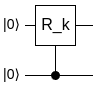
\includegraphics[scale = 0.5]{images/5.4.png}
    
\end{minipage}
\begin{minipage}{0.1\textwidth}
    $=$
\end{minipage}
\begin{minipage}{0.5\textwidth}
       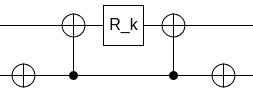
\includegraphics[scale = 0.5]{images/5.4.1.png}
\end{minipage}

as one can see by inputting the computational basis